% Template created by Adrienne Traxler (adrienne.traxler@wright.edu)
% Last modified: 3/22/17: Add clarifying note about why the template has too much space around its section headers.
% 
% Changelog
% 3/14/17: add 2-column figure example, tweak text to align with Word sample file, add hyperref for links/cross-references
% 6/21/16: 	Fix old PACS option and superscript affiliations.
% 5/5/16: 	Update sample table to use the REVTEX ruledtabular environment for auto-sizing;
%   		switch to using pra option until the prstper style is fixed (who knows when).
% 5/10/16: Swap suggested department/institution ordering in \affiliation lines.
% 5/12/16: Remove PACS line (deprecated).
% 6/21/16:	Switch to noshowpacs and add superscriptaddress in documentclass options.
% 
% This is my best effort to follow the Physical Review style guide plus specific changes 
% required for PERC (mostly, omitting article titles in references). This version compiles 
% with pdfLaTeX alone; using a proper .bib file changes the bibliography part at the end 
% and would require running BibTex as well.
%
% Finally, there's extra padding around section headers if you compile the bare template. 
% I believe that's because LaTeX stretches its white space to keep the floats (tables and 
% figures) near their input locations. The excess spacing goes away when a normal amount 
% of body text is filled in.

% Big list of reference documentation is here: http://journals.aps.org/revtex, 
%  see especially the APS Author Guide PDF link.

% Notes on the revtex4-1 documentclass options used: 
%  reprint does the double-column, publication ready appearance
%  prstper style formats reference numbers incorrectly, fast fix is to use pra instead.
%  Add longbibliography option to show article titles (and see note in bibliography)

%\documentclass[english,aps,prstper,reprint,showpacs]{revtex4-1}   % This version should work (prstper option), but actually formats reference numbers incorrectly.
\documentclass[english,aps,pra,reprint,noshowpacs,superscriptaddress]{revtex4-1}   
% Using pra instead of prstper gives correct square-bracket (not superscript) reference formatting
\usepackage[T1]{fontenc}	% should generally be included for better accented-word behavior
\usepackage[latin9]{inputenc}	% should generally be included for better accent behavior
\usepackage{geometry}		% for controlling page margins
\geometry{verbose,tmargin=1in,bmargin=1in,lmargin=0.75in,rmargin=0.75in}	% define margins
\usepackage{graphicx}
\usepackage[above,below]{placeins}	% allows use of \FloatBar­rier command to force section barriers
\usepackage{times}
% Next three lines are optional, use the hyperref package to make URLs and reference links live.
\usepackage{hyperref}  
\hypersetup{colorlinks=true,urlcolor=blue,citecolor=blue,linkcolor=blue}   
\urlstyle{same}
\pagestyle{empty}			% page numbers added later, when compiling the whole proceedings
\begin{document}

\title{Paradigms in Physics 2.0}
\author{David Roundy}
\author{Liz Gire}
\author{Ethan Minot}
\author{Emily van Zee}
\affiliation{Department of Physics, Oregon State University, Corvallis, Oregon, 97331}
\author{Tevian Dray}
\affiliation{Department of Mathematics, Oregon State University, Corvallis, Oregon, 97331}
\author{Corinne A. Manogue}
\affiliation{Department of Physics, Oregon State University, Corvallis, Oregon, 97331}

%\keywords{}

\begin{abstract}
In 2016, the Department of Physics at Oregon State University began a
process to revise our Paradigms in Physics curriculum for physics
majors.  This poster will describe both the process by which our
department achieved consensus on this curricular change, and the
resulting curriculum.  The Paradigms 2.0 committee begain with a
survey of students and faculty, followed by individual interviews with
the faculty teaching each existing course.  As we developed a plan to
address student- and faculty-identified challenges in the curriculum,
we met with each faculty member individually to explain and refine our
proposal, which was unanimously approved by the faculty.  Major
changes include elimination or major changes to several courses (math
methods, computational physics, modern physics, electronics, and
classical mechanics), including the introduction of two sophomore-year
courses designed specifically to help prepare students to for their
upper-division courses.
\end{abstract}

\maketitle

\section{Introduction}
The Paradigms in Physics program

\subsection{Background}
\emph{What is the Paradigms now?}
\subsection{History of the Paradigms}
\emph{How did we get here?~\cite{manogue2001paradigms}}
\subsection{Motivation for the change}
There were a number of factors that motivated us to embark on the
Paradigms~2.0 process.  The original Paradigms in Physics curricular
reform from 200? was showing its age.  In the intervening years we
have made a large number of modifications, such as reordering
Paradigms, introducing one new Paradigm, and introducing and changing
computational physics courses.

\paragraph{Transfer students}
Our curriculum is strongly affected by our desire to accomodate
transfer students from community colleges.  This leads us to focus on
a physics major in which all upper-division courses are taken in two
years.  However, our current curriculum is very hard on students in
the fall of their junior year, and especially so for transfer
students.  So we hoped to structure the courses such that non-transfer
students could be better prepared for their junior year, while
transfer students could postpone a few courses so that their junior
Fall would be no more difficult than that of any other student.

\paragraph{Coupled curricular changes}
A backlog of curricular changes have accumulated that could not be
separated from an examination of the curriculum as a whole.  Most
notable were discussions of the requirements for computational
physics, the amount of required electronics credits, and the role of
our modern physics course.  These persistent issues were not easily
addressed without addressing the physics major curriculum as a whole,
and any discussion of one tended to devolve into a discussion of
everything, without progress being made.

\paragraph{New faculty}
At this stage, (XX) of our faculty was not present during the orignal
Paradigms effort.  Many of the newer faculty have only a superficial
undertanding of our course structure.  This poses a challenge when
these professors teach courses that are closely intertwined with one
another.

\section{Paradigms 2.0 process}
\emph{How did we do it?}

%\newcommand\mathcourse[2]{\emph{#1 (#2)}}
\newcommand\mathcourse[2]{\emph{#1}}
\newcommand\noted[2]{\textbf{#1} (#2)}
\newcommand\paradigm[1]{{\sc #1} (3)}
\newcommand\capstone[1]{#1 (3)}
\newcommand\onecredit[1]{#1 (1)}
\newcommand\threecredit[1]{#1 (3)}
\newcommand\fourcredit[1]{#1 (4)}

\begin{figure*}
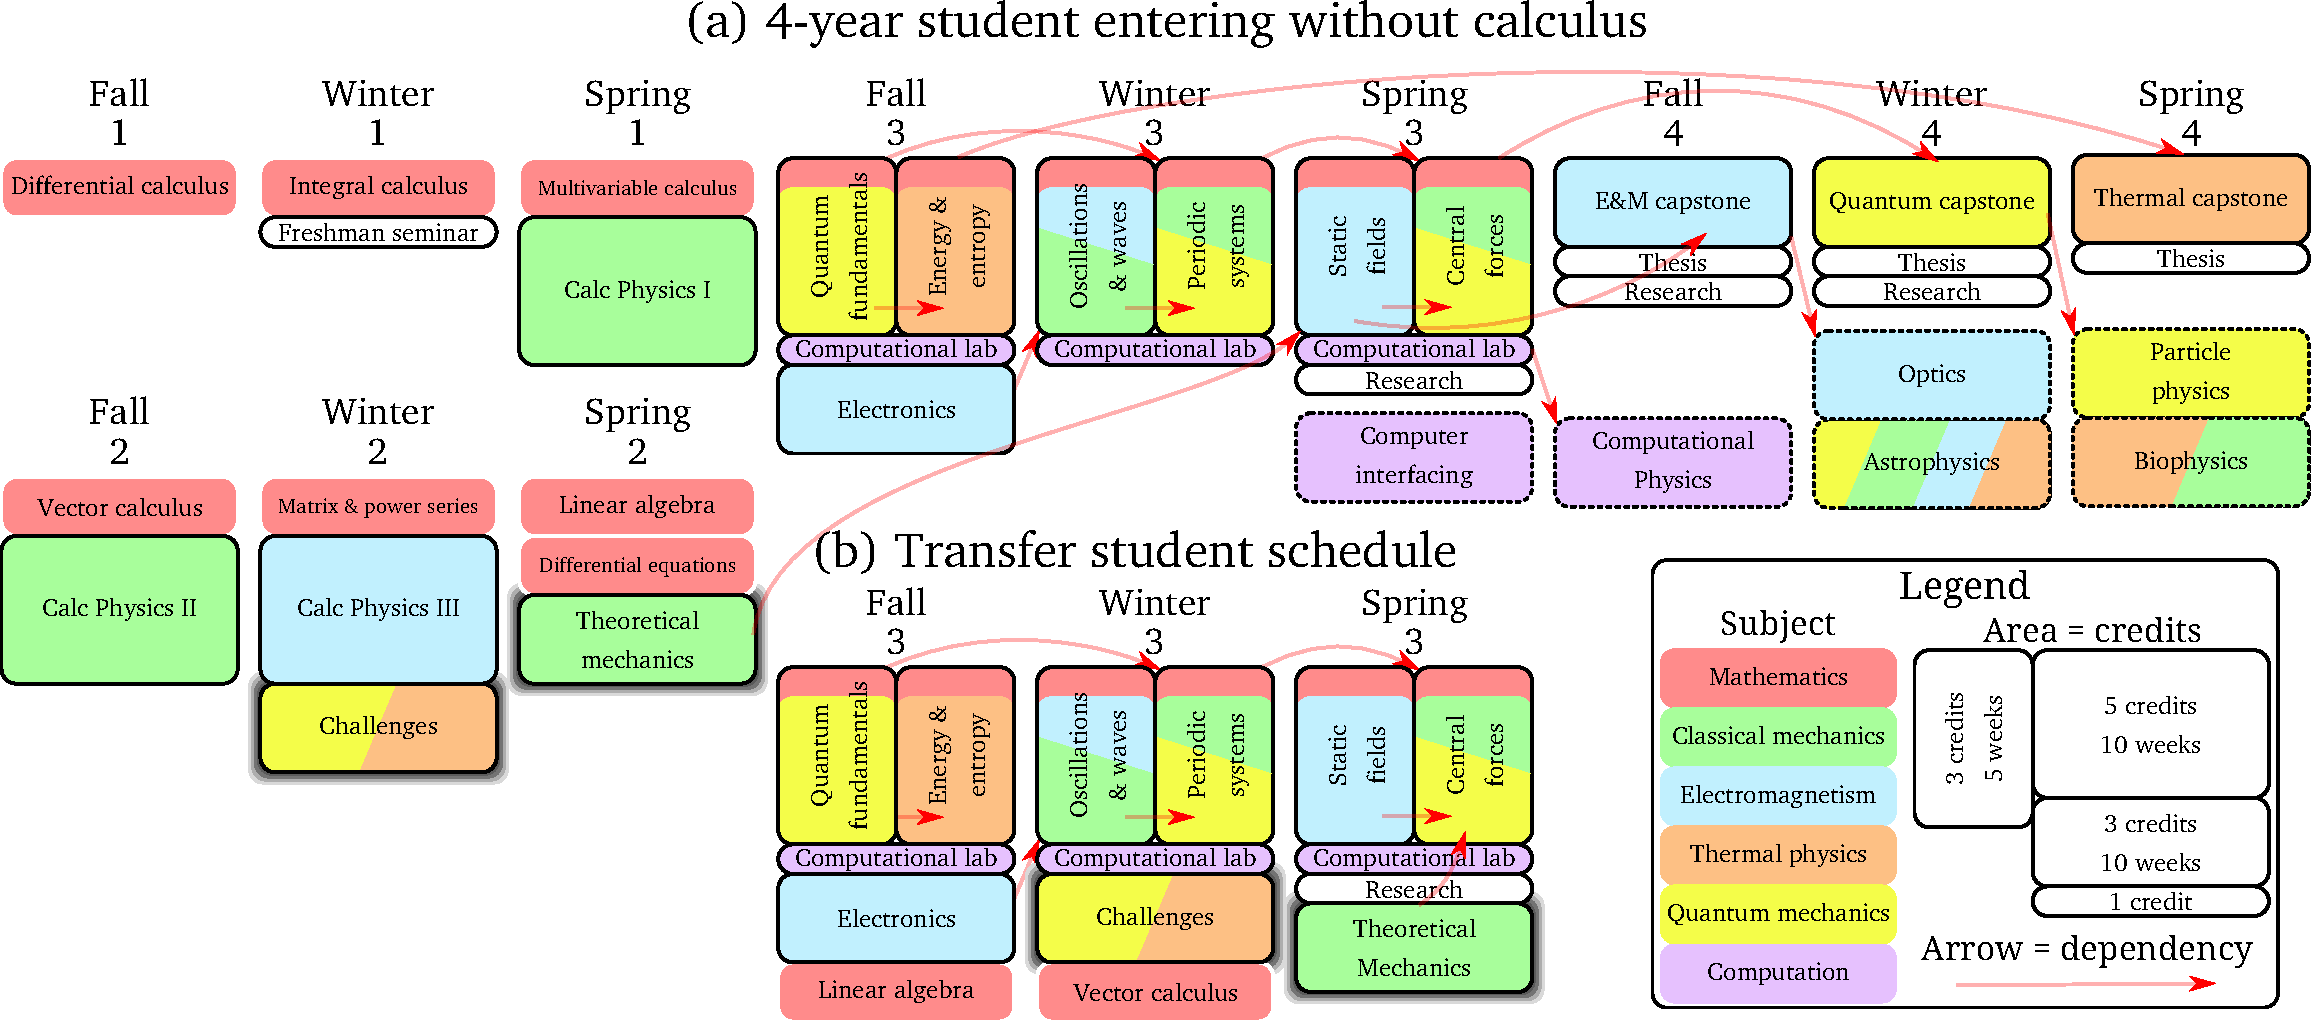
\includegraphics[width=\textwidth]{schedule}
\caption{Hypothetical student schedules for (a) a student entering
  without calculus and (b) a transfer student.  The Dependencies
  between courses are noted with arrows.  The area of each course is
  proportional to the credit value of the course, with the exception
  of math courses, which are shown in small boxes even though they are
  4-credit courses.  The two newly introduced courses are indicated
  with shadows.\label{fig:schedule}}
\end{figure*}

\section{Changes made}
As a result of this process, we have implemented a number of changes
to our physics major curriculum.  The resulting curriculum is outlined
in Fig.~\ref{fig:schedule}.  The changes consisted of introducing two
new sophomore-level courses (which may be taken in the junior year) to
better prepare our majors for the Paradigms.  We eliminated Modern
Physics and the Classical Mechanics capstone in favor of the two new
sophomore-level courses.  We eliminated the Math Methods course in
favor of ``math bits'' integrated into the Paradigms themselves.
Finally, we restructured our nine 3-week Paradigms courses into six
5-week Paradigms.  We changed our computational physics requirement,
and reduced the number of electronics courses.

\subsection{5-week Paradigms}
To begin with the most distinctive feature of our curriculum, we
wanted to maintain the existing intensive 7-hour-per-week schedule in
the junior year, which we have found effective.  However, we chose to
change from three 3-week Paradigms per quarter to two 5-week Paradigms
per quarter.    This change has several advantages.  It gives students
a bit more time with each professor prior to their final exam.  This
gives a bit more flexibility, for instance, in case of illness.
Finally, by reducing the number of Paradigms, we allow the curriculum
to be taught with fewer faculty, albeit at a work load per professor.

We put considerable thought into the content and ordering of the new
Paradigms.  In most cases, we think of each 5-week Paradigm as either
one formerly 4-week Paradigm (the one that consumed the extra week
each quarter) or two 3-week Paradigms compressed.  The major
scheduling change is to place Static Fields (electrostatics and
magnetostatics) in the spring quarter.  This intended to give students
a bit more time to take Vector Calculus.  It also puts all use of
curvilinear coordinates in the spring quarter, which should ease the
learning of Central Forces.  The final major change was the
elimination of special relativity from the Paradigms, which is has now
moved into the new sophomore-level Theoretical Mechanics course.

\subsection{Math bits}
We chose to eliminate the Math Methods course in favor of formal
``math bits'' in the Paradigms.  Our previous Math Methods Capstone
posed a challenge regarding placement in the curriculum: it needed to
be sufficiently late in order for students to be adequately prepared
for advanced mathematical content, but in order to be functional in
the curriculum it should teach content that is required by other
physics courses, and thus should be earlier in the curriculum.  In
response to these issues, and in recognition that the majority of our
majors are not bound for graduate school, and have no need for
advanced math methods, we chose to integrate the needed math content
into the Paradigms, and allow advanced students to take our
graduate-level Math Methods course.  In order to ensure that our
students to receive the math instruction they require, and based on
our previous experience with math-intensive weeks (the ``odd'' weeks)
in the Paradigms, we chose to integrate one week of ``math bits'' into
each Paradigm.  The math bits for the entire year are treated as a
distinct teaching assignment, so students will be accustomed to the
treatment of math as a distinct subject supporting the physics
content.  This provides some relief from teaching for the Paradigms
professors, and at the same time ensures that they do not succumb to
the temptation to short-change the math content to the detriment of
the students.

\subsection{Electronics}
We chose to reduce the Electronics requirement from two 3-credit
courses to one 3-credit course.  For many physics majors, this is more
than sufficient, and gives students a greater number of electives.  In
addition, we removed the lecture section of this course---which had
developed an unusually high student work load for a 3-credit
course---in favor of in-lab instruction.

A final change to Electronics is that we now will \emph{require}
Electronics during the junior year (specifically as a prerequisite for
Oscillations and Waves).  This is made possible by the reduction in
Fall workload for incoming transfer students, who had previously
usually taken Electronics as a senior.  This change has enabled us to
articulate distinct and sequenced learning outcomes from these two
courses, particularly in the realm of complex exponentials and Fourier
transforms.  It is also beneficial in providing students with
trouble-shooting skills prior to the in-class labs taught in
Oscillations and Waves.

\subsection{Computational lab}
Over the last six years, we have been developing a 1-credit
computational laboratory course that accompanies the Paradigms.  We
chose to require this course, while removing a requirement for a
lower-division 3-credit course in computational physics.  This
lower-division course was challenging to teach, since it always had a
mix of lower- and upper-division students, with very different skill
levels and needs.  Transfer students now take computation alongside
the non-transfer students, in a laboratory setting using pair
programming to help new programmers to learn.

\subsection{Sophomore courses}
We introduced two new sophomore-level courses: \emph{Challenges in
  Contemporary Physics}, and \emph{Theoretical Mechanics}.  Both of
these courses are designed to ramp up student mathematical abilities
prior to their junior year.  The Challenges course will focus on
estimation, dimensional reasoning, and interpretation of integrals,
while Theoretical Mechanics will teach power series approximations,
and expose students to increased levels of mathematical
sophistication.

These courses \emph{will} have the challenge (which was removed from
the computational course!) of teaching both juniors and sophomores
together.  They will be taught in the winter and spring quarters, so
as to reduce the burden on transfer students in the Fall.  They were
explicitly constructed to \emph{not} teach any content required for
Fall or Winter Paradigms so that they can be taken concurrently with
the Paradigms.

\subsubsection{Challenges in Contemporary Physics}
\emph{Course overview: relevant to world, benefit for diversity and
  recruitment, replaces Modern Physics. Topics.}
\subsubsection{Techniques of Theoretical Mechanics}
\emph{Course overview: special relativity, rocket motion, Lagrangian
  mechanics.}

\section{Outcomes}
\emph{How has it gone?}

\subsection{Faculty vote}
\emph{Unanimous result.}
\subsection{Transition year}
\emph{Gradual transition, getting courses taught.}

\section{Future research}
\emph{Document learning trajectories, new courses.}

% Formatting tweak if needed--FloatBarrier forces floats to show here, before next section
%\FloatBarrier	


\section{Conclusions}
\emph{We made some changes, and the process went well.}

\acknowledgments{Put references below the acknowledgements (and appendixes, if any).}

% For a longer bibliography, delete the thebibliography block above, then comment in 
% these two lines to use a .bib file with BibTeX.
\bibliographystyle{apsrev}  	% supercedes the longbibliography option, so leave commented out if you want to display article titles
\bibliography{paper}  	% don't include the .bib suffix

\begin{table*}[htbp]
\caption{Hypothetical student schedule for a student entering without
  calculus.  Students with AP Calculus can take the junior-year
  courses one year earlier, and students who start calculus-based
  physics in the Fall of their second year are not
  delayed.\label{schedule}}
\begin{ruledtabular}
\begin{tabular}{rlll}
  \textbf{Year} & \textbf{Fall} & \textbf{Winter} & \textbf{Spring} \\
  \hline
  1 & \mathcourse{Differential calculus}{251} &
  \mathcourse{Integral calculus}{252} &
  \mathcourse{Multivariable calculus}{254} \\
    & & \onecredit{Freshman Seminar} & \fourcredit{Calc Physics I} \\
\hline  2 & \mathcourse{Vector calculus}{255}
  & \mathcourse{Differential equations}{256}
  & \mathcourse{Linear algebra}{341} \\
  & \fourcredit{Calc Physics II} & \fourcredit{Calc Physics III} &\mathcourse{Series \&
    sequences}{253} \\
  && \noted{Challenges}{3} & \noted{Theoretical Mechanics}{3}
  \\
\hline 3 & \paradigm{Quantum fundamentals} & \paradigm{Osciallations \& waves} & \paradigm{Static fields}
\\
  & \paradigm{Energy \& entropy} & \paradigm{Periodic systems} & \paradigm{Central forces}
\\
  & \onecredit{Computational lab I} & \onecredit{Computational lab II} & \onecredit{Computational lab III}
\\
  & \threecredit{Electronics} & \threecredit{Computer interfacing} & \onecredit{Research}
\\
\hline 4 & \capstone{Electromagnetism capstone} & \capstone{Quantum capstone} & \capstone{Thermal capstone}
\\
& \onecredit{Thesis} & \onecredit{Thesis} & \onecredit{Thesis}
\\
& \onecredit{Research} & \onecredit{Research}
\end{tabular}
\end{ruledtabular}
\end{table*}

\begin{table*}[htbp]
\caption{Hypothetical transfer student schedule.  Most transfer
  students will have a heavier schedule in their transfer year due
  to need to catch up on required math courses.\label{schedule}}
\begin{ruledtabular}
\begin{tabular}{rlll}
  \textbf{Year} & \textbf{Fall} & \textbf{Winter} & \textbf{Spring} \\
  \hline
3 & \paradigm{Quantum fundamentals} & \paradigm{Osciallations \& waves} & \paradigm{Static fields}
\\
  & \paradigm{Energy \& entropy} & \paradigm{Periodic systems} & \paradigm{Central forces}
\\
  & \onecredit{Computational lab I} & \onecredit{Computational lab II} & \onecredit{Computational lab III}
\\
  & \threecredit{Electronics} & \threecredit{Computer interfacing} & \onecredit{Research}
\\
& \mathcourse{Linear algebra}{341} & \noted{Challenges}{3} & \noted{Theoretical Mechanics}{3}
\\
&&\mathcourse{Vector calculus}{255}
\\
\hline 4 & \capstone{Electromagnetism capstone} & \capstone{Quantum capstone} & \capstone{Thermal capstone}
\\
& \onecredit{Thesis} & \onecredit{Thesis} & \onecredit{Thesis}
\\
& \onecredit{Research} & \onecredit{Research}
\end{tabular}
\end{ruledtabular}
\end{table*}

\end{document}
